%--------------------------------------------------------------
\section{StretchMapping: create 1D stretching functions}
\index{stretch mapping}\index{Mapping!StretchMapping}
%-------------------------------------------------------------

The StretchMapping class, derived from the Mapping Class can be used
to define one-dimensional ``stretching'' functions. These functions
are often used to stretch grid lines on existing Mappings. These
functions can also be used as a blending function for the {\tt TFIMapping}.

There are several types of stretching functions:

\subsection{Inverse hyperbolic tangent stretching function}\index{stretching!inverse hyperbolic tangent}

This stretching function is a one-dimensional map
from $r$ into $x$ defined (in an inverse fashion) by
$$
r = R(x) = \Big[ x + \sum_{i=1}^{nu} ( U_i(x)-U_i(0) )
                   + \sum_{j=1}^{nv} ( V_j(x)-V_j(0) ) \Big] \times {\rm scale}+ {\rm origin}
$$
where $U_i(x)$ is a ``layer'' function
$$
    U_i(x) = {a_i\over 2} \tanh b_i(x-c_i)
$$
and $V_i(x)$ is an ``interval'' function
$$
    V_j(x) = {d_j-1 \over 2} \log\left( 
          \cosh e_j (x-f_j) \over
          \cosh e_j (x-f_{j+1}) \right) {1 \over 2 e_j}
$$

The stretching mapping is often used to stretch grid points in parameter
space.
The functions $U_i$ are used to concentrate grid points in at a point
while the functions $V_j$ are used to transition from one grid spacing
to another. When the mapping is invertible a spline can be fitted 
to the inverse to be used as an initial guess for Netwon. Usually only
$1$-$3$ Netwon iterations are needed.



Here the terms ${\rm scale}$ and ${\rm origin}$ are normalization factors determined so 
that $R(0) = 0$ and $R(1) = 1$.  The remaining parameters are input by
the user and have the following constraints:
\begin{eqnarray*}
                  b_j &>& 0, ~~j=1,..,n_u,      \\
           0 \leq c_j &\leq& 1,  ~~j=1,..,n_u, \\
                  e_j &>& 0, ~~ j=1,..,n_v,    \\
  f_1 \leq 1,~~f_{n_v} &\geq& 0,~~\leq f_j \leq 1,
       ~~~~j=2,..,n_v-1,  ~~~~ {\rm and}  \\
      f_1 < f_2 < f_3 &<& ... < f_{n_v}.
\end{eqnarray*}
\vskip\baselineskip

\noindent
The function $U_i(x)$ is a hyperbolic tangent that is
centered at
$x=c_i$ and asymptotes to $-a_i/2$ or $a_i/2$ (see Figure~\ref{fig:stretchV}).
As $b_i$
tends to infinity,
the function $U$ tends toward a step function.

The function $V_j(x)$ (which is the integral of the difference between
two layer functions) is a smoothed-out ramp function with transitions
at $f_j$ and $f_{j+1}$ (see Figure~\ref{fig:stretchV}).  The slope of the
ramp is $d_{j-1}$.  Thus $d_j$ indicates the relative slope of the
ramp compared to the linear term ``$x$,'' which appears in $R(x)$.
That is, if $d_j=2$, then the slope of $R(x)$ between $f_j$ and
$f_{j+1}$ will be approximately twice the slope of the region where
the linear term is dominant.  A sloped region can be made to extend
past $x=0$ or $x=1$ (so that $x=0$ or $x=1$ is in the middle of the
sloped region) by choosing $f_1<0$ or $f_{n_v+1}>1$.  A reasonable
value might be $f_1=-.5$ or $f_{n_v+1}=1.5$.  Note that when a grid is
periodic in the $r$- direction, the functions $U_i(x)$ and $V_j(x)$
are replaced by functions $U^p_i(x)$ and $V^p_j(x)$, respectively,
which are given by
$$
 U^p_i(x) = \sum_{k = -\infty}^{+\infty} U_i(t+k),        ~~~
 V^p_j(x) =  \sum_{k = -\infty}^{+\infty} V_j(t+k).
$$
These functions are not really periodic, but their derivatives
with respect to $x$ are periodic with period 1.
%- \begin{figure}
%-   \includegraphics[width=9cm]{\figures/stretchU}
%-   % \epsfig{file=\figures/stretchU.ps,bbllx=60,bblly=150,bburx=250,bbury=392}  % (238,392), (576,784)
%-   \caption{The `layer' function $U(t)$ for concentrating grid lines at a point. The grid spacing
%-       is smaller where the slope is larger.}  \label{fig:stretchU}
%- \end{figure}
%- 
\begin{figure}[hbt]
\newcommand{\figWidth}{12cm}
\newcommand{\trimfig}[2]{\trimFig{#1}{#2}{0.1}{.1}{.25}{.6}}
\begin{center}\small
% ------------------------------------------------------------------------------------------------
\begin{tikzpicture}
  \useasboundingbox (0,0.) rectangle (12,6);  % set the bounding box (so we have less surrounding white space)
% 
  \draw (0, 0) node[anchor=south west,xshift=-4pt,yshift=-4pt] {\trimfig{\figures/stretchU}{\figWidth}};
% grid:
%   \draw[step=1cm,gray] (0,0) grid (12,6);
\end{tikzpicture}
% ----------------------------------------------------------------------------------------
  \caption{The `layer' function $U(t)$ for concentrating grid lines at a point. The grid spacing
      is smaller where the slope is larger.}  \label{fig:stretchU}
\end{center}
\end{figure}

The following remarks may prove useful in making choices for the
parameters $a_i, ... ,f_i$.  Below, the variable $r$ typically refers
to a uniform grid, while $x$ refers to a grid that has been stretched
so that points are clustered in certain locations on the $x$ axis.
The clustering of points can be done in two ways.  Using the $U_i(x)$
functions (tanh's), the point spacing can be made to decrease
exponentially to a minimum spacing at $c_i$.  The value of $b_i$
determines how small the spacing can get.  Roughly speaking, a value
of $b_i=10.0$ means the spacing will be about 10 times smaller at the
center of the layer than in the unstretched parts of the grid.  The
relative number of points in this stretched region is proportional to
$a_i$.  The linear term $x$ appearing in the definition of $R(x)$ has
a weight of one (1), so if there is only one term $U_i(x)$, the
relative number of points in the layer is essentially $a_1 / (1+a_1)$.
Thus, if $n_u=1$, ($n_v=0$), and $a_1=1$, then half the points will be
in the stretched layer.  For two layers, the relative number of points
in layer $i$ ($i=1$ or $i=2$) is $ a_i / (1+a_1+a_2)$.
\begin{figure}[hbt]
\newcommand{\figWidth}{12cm}
\newcommand{\trimfig}[2]{\trimFig{#1}{#2}{0.1}{.1}{.175}{.6}}
\begin{center}\small
% ------------------------------------------------------------------------------------------------
\begin{tikzpicture}
  \useasboundingbox (0,.5) rectangle (12,7);  % set the bounding box (so we have less surrounding white space)
% 
  \draw (0, 0) node[anchor=south west,xshift=-4pt,yshift=-4pt] {\trimfig{\figures/stretchV}{\figWidth}};
% grid:
%   \draw[step=1cm,gray] (0,0) grid (12,7);
\end{tikzpicture}
% ----------------------------------------------------------------------------------------
  \caption{The `ramp' function $V(t)$ for changing from one grid spacing to another. The grid spacing
      is smaller where the slope is larger.} \label{fig:stretchV}
\end{center}
\end{figure}
%- \begin{figure}
%-   \includegraphics[width=9cm]{\figures/stretchV}
%-   % \epsfig{file=\figures/stretchV.ps,width=2.25in,bbllx=30,bblly=150,bburx=250,bbury=375}
%-   \caption{The `ramp' function $V(t)$ for changing from one grid spacing to another. The grid spacing
%-       is smaller where the slope is larger.} \label{fig:stretchV}
%- \end{figure}
The functions $V_j(x)$ allow you to have intervals where the grid
point spacing is relatively smaller or larger than the grid spacing in
the region where the linear term $x$ is dominant.  In each interval,
the grid spacing is nearly constant, except near the transition points
$f_i$ and $f_{i+1}$.  The parameter $d_i$ denotes the relative grid
spacing in each interval.  For example, to make the grid spacing twice
as fine for t between 0.25 and 0.5, you would specify $f_1=0.25$,
$f_2=0.5$, and $d_1=2$.  As another example, to make the spacing 5
times smaller for $x$ between 0 and 0.5, you could say $f_1=-0.5$,
$f_2=0.5$, and
$d_1=5$.  Assigning the first transition point a value less than zero,
$f_1=-0.5$, means that $x=0$ will be in the middle of the interval
where the spacing will be 5 times smaller.  (If instead $f_1=0 $, then
near $t=0 $ the spacing would be in transition to the default relative
grid spacing of 1).  The parameters $e_i$ denote how rapid the
transition is from one spacing to another.  A reasonable value for
$e_i$ might be 10.0 or 20.0. 

% Various examples of stretching functions are shown in Figure~\ref{figstr}.

Figure~\ref{fig:itanhStretch} shows an example of using the inverse hyperbolic tangent function
to stretch grid lines on a square.
\begin{figure}
  \begin{center}
  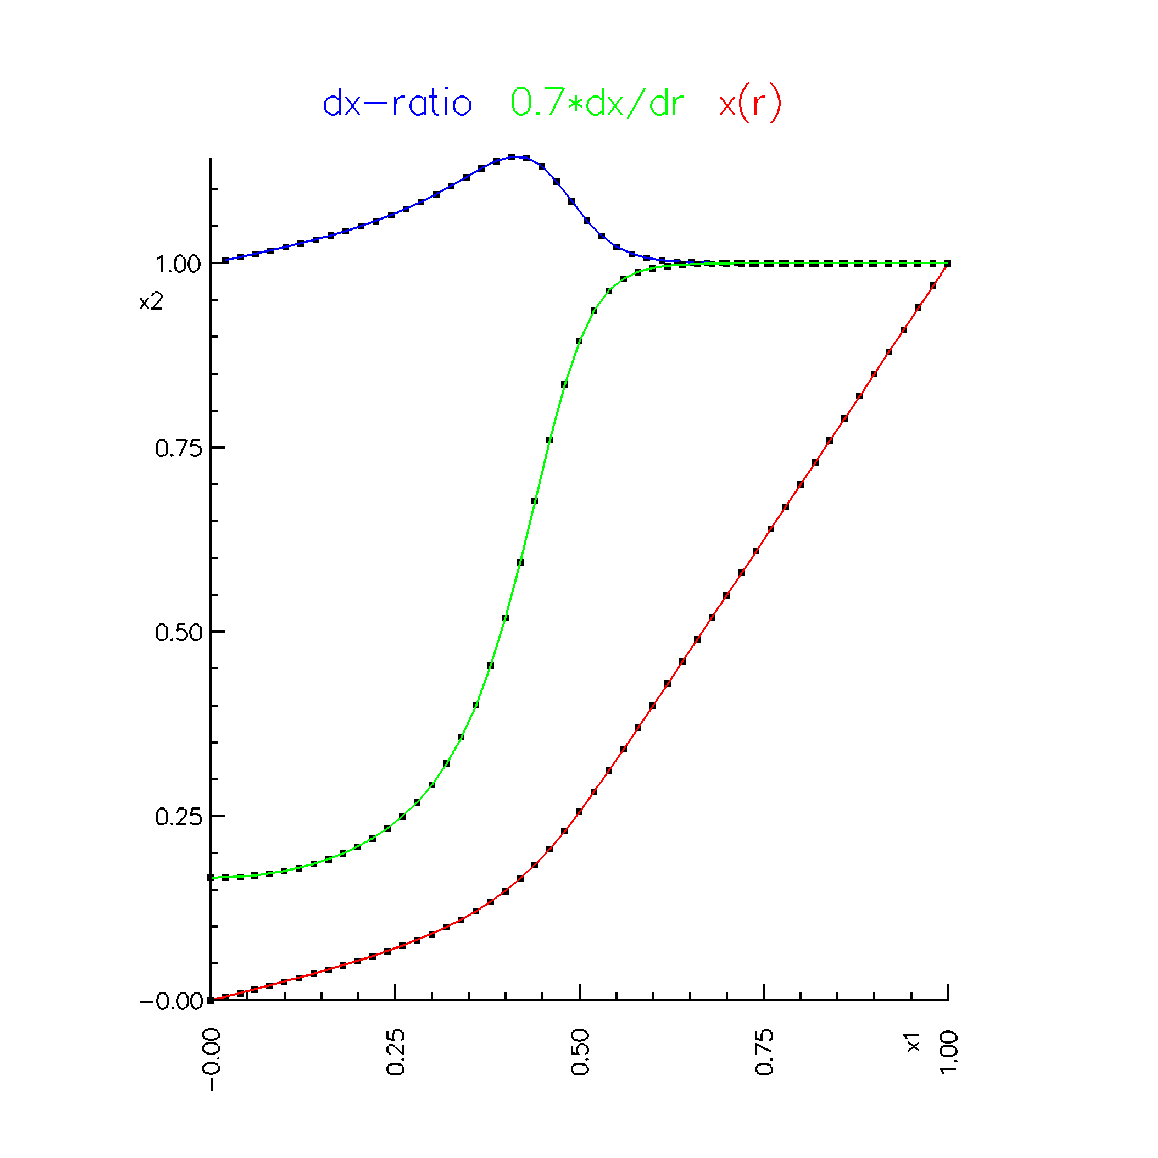
\includegraphics[width=8cm]{\figures/itanhCurves}
  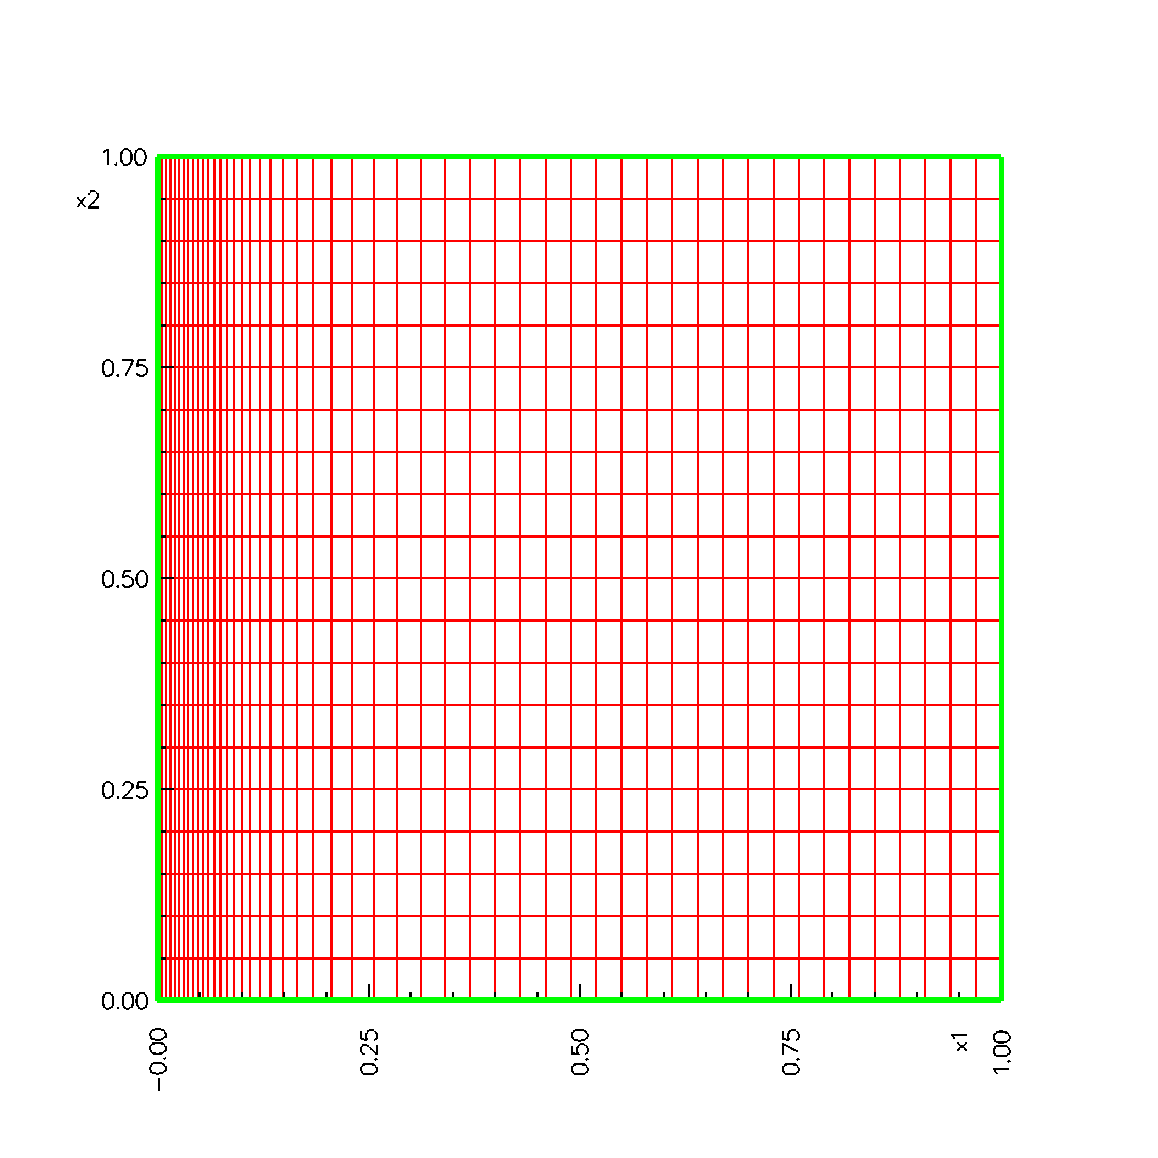
\includegraphics[width=8cm]{\figures/itanhSquare}
  \end{center}
  \caption{The inverse hyperbolic tangent stretching function (red curve on left) used to cluster grid points on a square.}\label{fig:itanhStretch}
\end{figure}


\subsection{Hyperbolic tangent stretching function}\index{stretching!hyperbolic tangent}

This function is defined as
$$
    x(r) = \left\{ a_0 + a_r r + a_1 \tanh( b_1(r-c_1) ) + origin \right\} scale
$$
If the function is normalized (optional) then origin and scale are chosen to that $x(0)=0$ and $x(1)=1$. 
Note that $a_1$ will normally be negative in order to concentrate lines near $r=c_1$.
To be invertible one should choose $a_r > -a_1 b_1$ 
(a sufficient but not necessary condition).

Figure~\ref{fig:itanhStretch} shows an example of using the hyperbolic tangent function
to stretch grid lines on a square.
\begin{figure}
  \begin{center}
  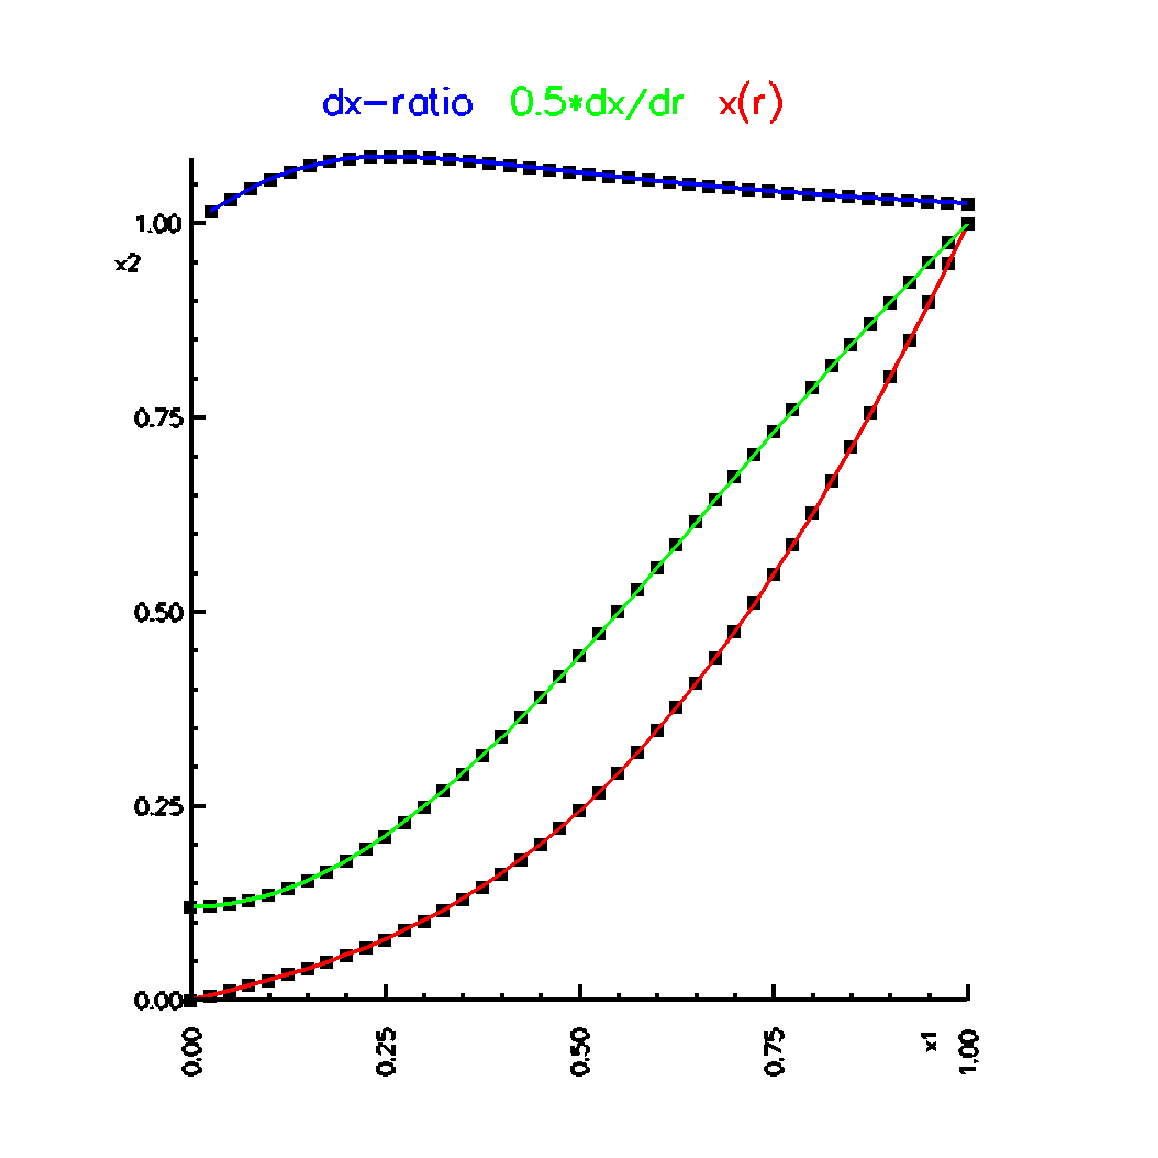
\includegraphics[width=8cm]{\figures/tanhCurves}
  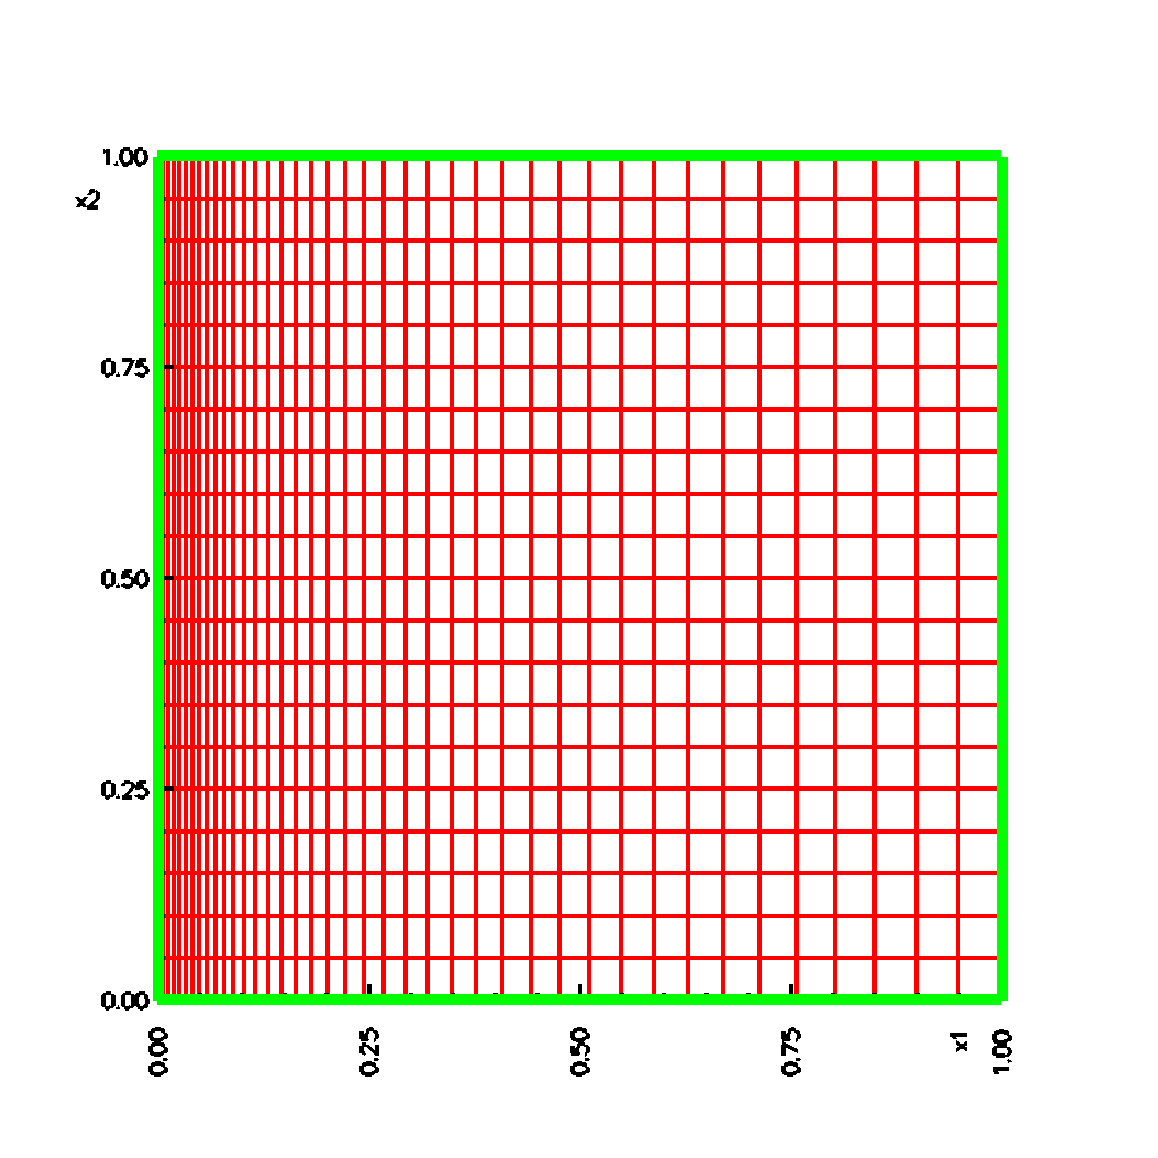
\includegraphics[width=8cm]{\figures/tanhSquare}
  \end{center}
  \caption{The hyperbolic tangent stretching function (red curve on left) used to cluster grid points on a square.}\label{fig:itanhStretch}
\end{figure}


\subsection{Exponential stretching function}\index{stretching!exponential}

This function is defined as
$$
    x(r) = \left\{ a_0 + a_r r + a_1\exp( b_1(r-c_1) ) + origin  \right\} scale
$$
If the function is normalized (optional) then origin and scale are chosen to that $x(0)=0$ and $x(1)=1$. 

\subsection{Exponential blending function}\index{stretching!exponential blend}

This function is defined as
\[
  x(r) = \left \{\begin{array}{lr}
 1 & {3\over4} \le s \le 1\\
 \left[1 + \exp\left(-{\displaystyle\sqrt3\over\displaystyle4}
   {\displaystyle2s-1\over
     ({\displaystyle s-}{1\over4})
     ({3\over4}{\displaystyle -s})}\right)\right]^{-1}
 & {1\over4}<s<{3\over4} \\
 0 & 0 \le s \le {1\over4} \\
 \end{array} \right.
\]
This function is used by the {\tt FilletMapping} in order to make a smooth curve
in the region where two curves intersect.



\subsection{Exponential to Linear function}\index{stretching!exponential to linear}

The exponential to linear stretching function can be used to transition between
an exponentially streched grid at one boundary and a uniform distribution of
points at the opposite boundary as shown in Figure~\ref{fig:expLinear}. (The version of this
function for stretching at an interior point is described below).
This stretching function is defined as 
\begin{equation}
  x(r) = \left\{ \log( 1 + a e^{s b (r-c)} )  - x_0 \right\} d 
\end{equation}
where $x_0$ and $d$ are chosen so that $x(0)=0$ and $x(1)=1$. The parameter $c$
takes the values $c=0$ and $c=1$ to stretch at $r=0$ or $r=1$. The parameter $s$ is $+1$ or $-1$ depending on $c$, $s=1-2c$.
The parameter $a$ is normally taken to be small and is approximately the ratio of the finest
grid spacing to the largest grid spacing. 
The derivative of this stretching function is 
\begin{align*}
  x_r(r) & = \left\{ { a s b e^{s b (r-c)} \over  1 + a e^{s b (r-c)}} \right\} d,  \\
         & = (s b d)~ \phi(a e^{s b (r-c)}),     \\
  \phi(y) & = { y \over 1 + y } .
\end{align*}
The grid spacing is $x_r(r) \Delta r$ (where $\Delta r$ is the grid spacing in $r$) and for $a \ll 1 $,
\begin{align*}
  x_r(c) & \approx  (s b d) a  , \\
  x_r(1-c) & \approx (sb d)
\end{align*}
and thus the grid spacing at $r=c$ is a factor of $a$ times that at $r=1-c$.
The function $\phi(y)$ is used to transition between an exponentially increasing
grid spacing when $y=a e^{s b (r-c)}$ is small (since $\phi(y) \sim y$ for $y\ll 1$),
and a constant grid spacing for $y\gg 1$ (since $\phi(y) \sim 1$ for $y\gg 1$).
The parameter $b$ determines how fast the grid spacing increases near $r=c$. The grid spacings
will increase by a factor of about $e^{b \Delta r}$. Normally for PDE applications $b$ and $\Delta r$ should be
chosen so that the growth factor $\kappa = e^{b \Delta r}$
is not be too large or else the grid metrics change too rapidly resulting in lower accuracy. 
Typically $\kappa < 1.15$ for example. 
The parameter $b$ might usefully be chosen so that
$a e^b = B$ where $B$ is fairly large ($B\approx 10$) since then $\phi(B) \approx 1 - 1/B $ and thus
the function will be nearly linear at $r=1-c$. 

The exponential to linear stretching function was derived by first choosing $\phi(y)$
and then integrating to get $x(r)$. Besides the choice $\phi(y)=y/(1+y)$, 
$\phi$ could also be chosen as $\phi = \arctan(y)$ or $\phi=\tanh(y)$, for example.

\begin{figure}
  \begin{center}
    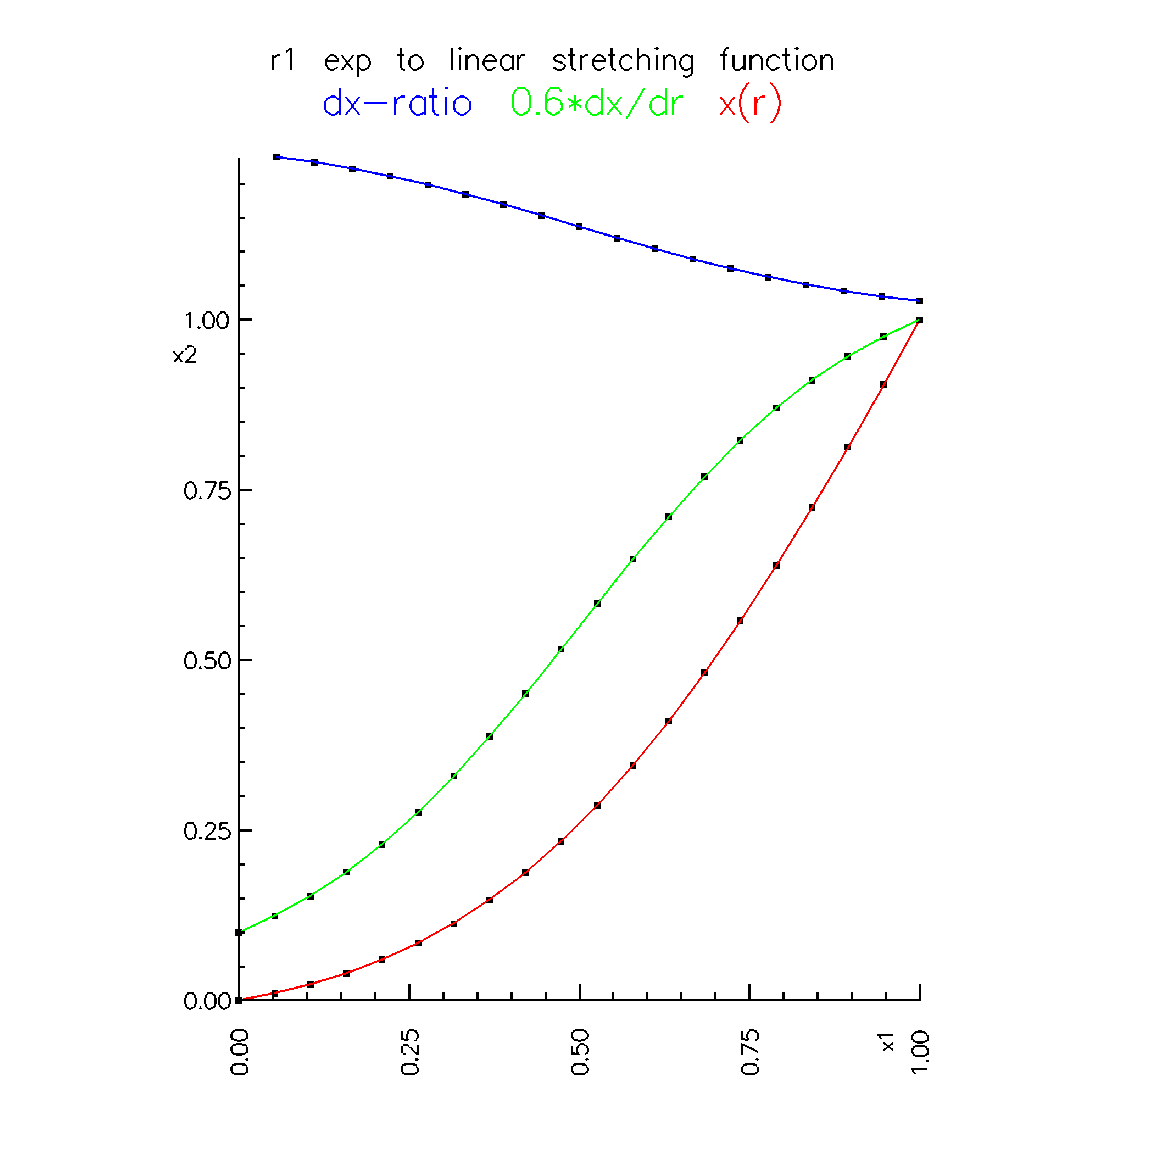
\includegraphics[width=8cm]{\figures/expLinearCurves}
    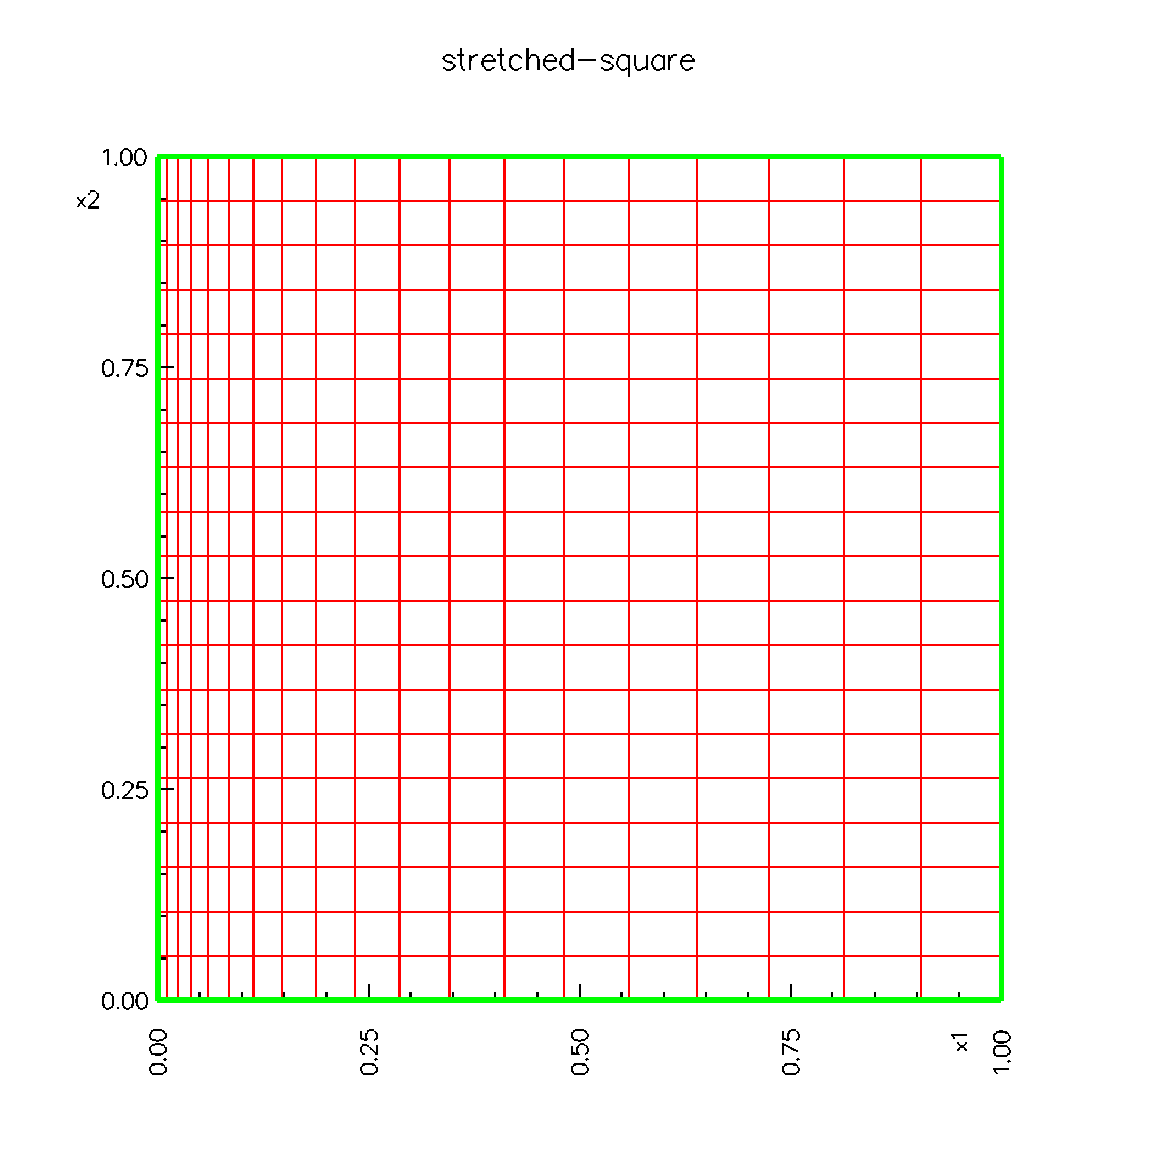
\includegraphics[width=8cm]{\figures/expLinearSquare}
  \end{center}
  \caption{The exponential to linear stretching function (red curve on left) transitions 
    from an exponential function to a linear function. The grid spacing increases exponentially near the left
    and transitions to a constant grid spacing on the right.} \label{fig:expLinear}
\end{figure}


The above exponential to linear stretching function can be extended to provide exponential stretching
at an interior point $c$ in the domain as shown in Figure~\ref{fig:expLinearInteruor}. In this case the function is defined by 
\begin{equation}
  x(r) = \left\{ \log\left( { 1 + a e^{b (r-c)} \over  1 + a e^{-b (r-c)} } \right)  - x_0 \right\} d 
\end{equation}
\begin{figure}
  \begin{center}
    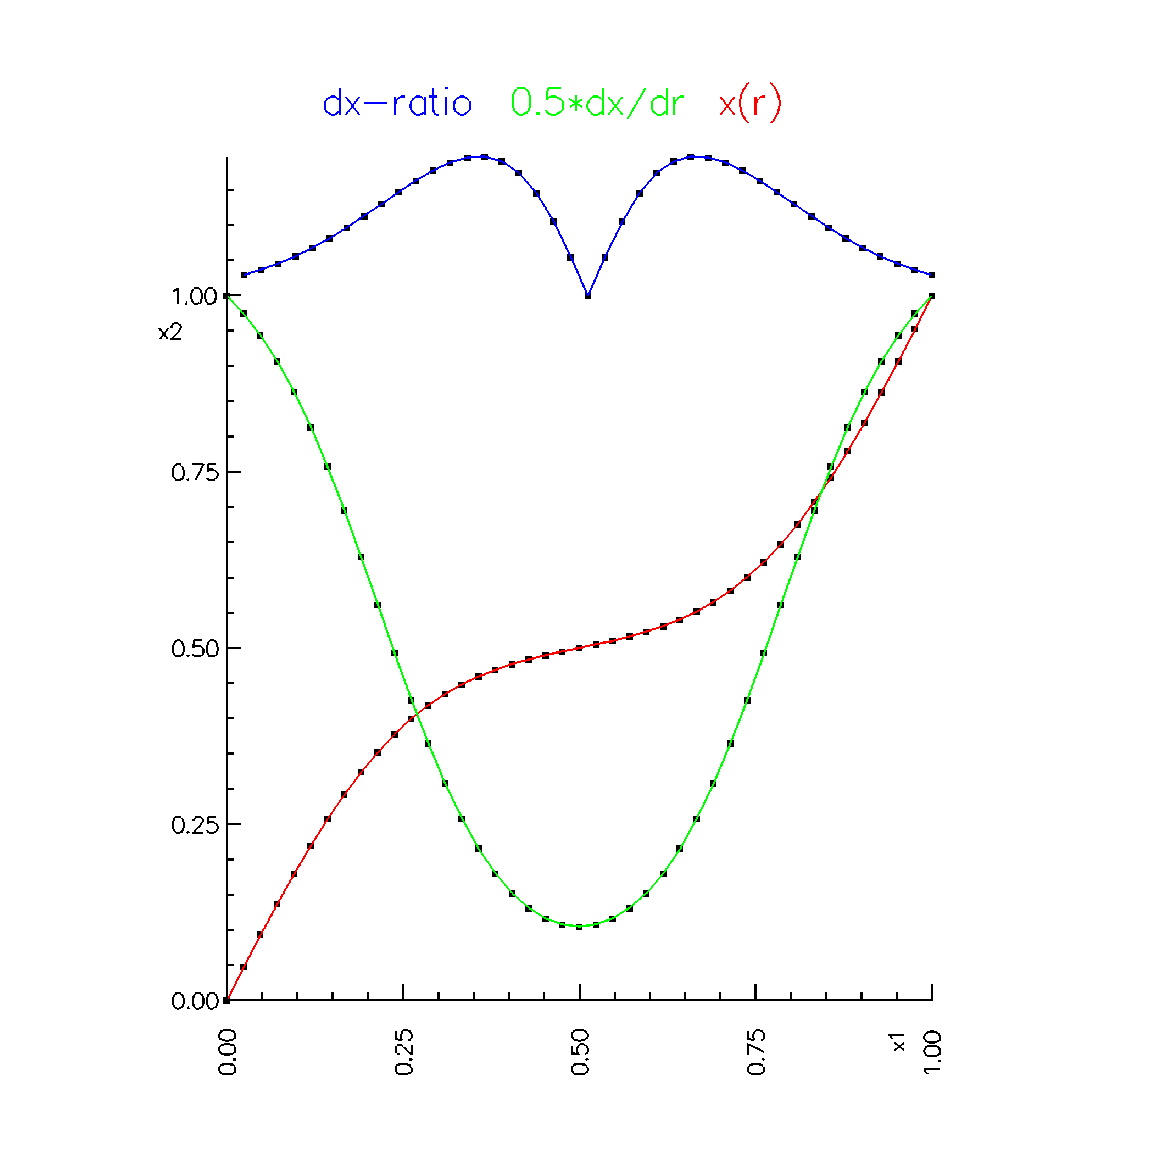
\includegraphics[width=8cm]{\figures/expLinearCurvesInterior}
    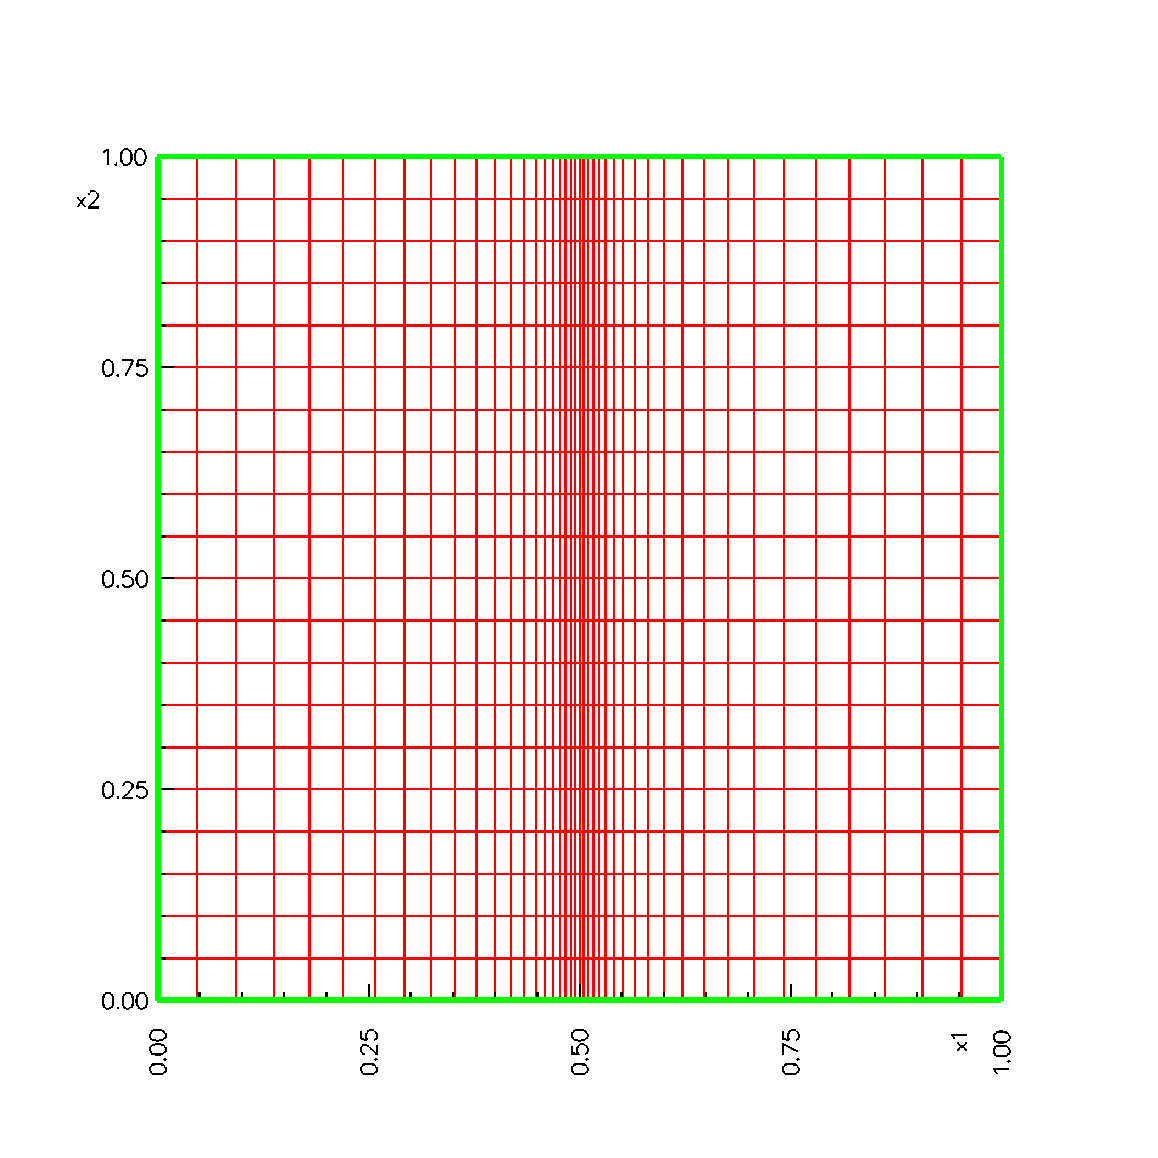
\includegraphics[width=8cm]{\figures/expLinearSquareInterior}
  \end{center}
  \caption{The exponentialToLinear stretching function for clustering points at an interior location.}
    \label{fig:expLinearInteruor}
\end{figure}


%% \subsection{Member function descriptions}
%% \input StretchMappingInclude.tex

% \subsection{Constructors}
% 
% % The arguments to the constructor indicate the number
% 
% \begin{tabbing}
% {\ff StretchMapping( int numberOfLayers=0, int numberOfIntervals=0 )xxxx}\= \kill
% {\ff StretchMapping( int numberOfLayers=0, int numberOfIntervals=0)}   
%     \> Constructor with defaults \\
% \end{tabbing}
% 
% 
% \subsection{Member Functions}
% 
% \begin{tabbing}
% 0123456789012345678901234567689012345678901234567890123 \= \kill
% {\ff void setNumberOfLayers( int numberOfLayers )}     
%        \> Change the number of Layers   \\
% {\ff void setNumberOfIntervals( int numberOfIntervals )}  
%        \> Change the number of Intervals    \\
% {\ff void setLayerParameters( int index, real a, real b, real c)}  
%        \>  set $(a,b,c)$ for $U_{index}$,
%                   $0\le {\ff index} < {\ff numberOfLayers}$ \\
% {\ff void setIntervalParameters( int index, real d, real e, real f)}  
%                \>  set $(d,e,f)$ for $V_{index}$
%                   $0\le {\ff index} < {\ff numberOfIntervals}+1$ \\
% {\ff void setNumberOfSplinePoints( int numberOfSplinePoints )}    
%               \> number of spline points used to compute ``inverse''   \\
% {\ff void setEndPoints( real rmin, real rmax )} 
%       \>  By default $0={\ff rmin} \le r \le {\ff rmax}=1$.  \\
% {\ff void setScaleParameters( real origin, real scale )} 
%       \>  Overide defaults ({\ff rmin}, {\ff rmax} not used) \\
% {\ff void setIsPeriodic( int trueOrFalse )} 
%       \>  Is the mapping periodic (TRUE/FALSE)? \\
% {\ff void map( ... )}  \> evaluate the mapping and derivative  \\
% {\ff void inverseMap( ... )}  \> evaluate the inverse mapping and derivative  \\
% {\ff void get( const Dir \& dir, const String \& name)} \> get from a database file \\
% {\ff void put( const Dir \& dir, const String \& name)} \> put to a database file \\
% \end{tabbing}
% There are two ways to scale the function $r=R(t)$. By default the
% function is scaled so that $R(0)=0$ and $R(1)=1$. One can also choose
% to have $R(0)={\ff rmin}$ and $R(1)={\ff rmax}$ or one can explicitly
% set the parameters {\ff origin} and {\ff scale} found in the definition
% of $R(t)$ above.


\subsection{Examples}

Here is an example of the use of the {\ff StretchMapping} class.
{\footnotesize
\begin{verbatim}
#include "Stretch.h"

void main()
{
  const int axis1 = 0;
  const int axis2 = 1;
  const int axis3 = 2;
  realArray r(1,3);
  realArray t(1,3);
  realArray tr(1,3,3);

  StretchMapping stretch1( 2, 0 );                   // two layers, zero intervals
  stretch1.setLayerParameters( 0, 1., 10., .25 );    // set layer 0, a,b,c
  stretch1.setLayerParameters( 1, 1., 10., .75 );    // set layer 1, a,b,c
  stretch1.setIsPeriodic(FALSE);                     // default is FALSE

  r(0,axis1)=.5;
  stretch1.map( r,t,tr );                            // evaluate


  StretchMapping stretch2( 0, 1 );                   // zero layers, one interval
  stretch2.setIntervalParameters( 0, 5., 20., .25 ); // spacing is smaller
  stretch2.setIntervalParameters( 1, 0.,  0., .75 ); // between .25 and .75
  stretch2.setIsPeriodic(FALSE);                     // default is FALSE
  
  r(0,axis1)=.25;
  stretch2.map( r,t,tr );                            // evaluate

}
\end{verbatim}
}

\noindent
\begin{minipage}{.475\linewidth}
  \begin{center}
   \includegraphics[width=9cm]{\figures/stretch1} \\
   % \epsfig{file=\figures/stretch1.ps,width=\linewidth}  \\
  {Stretching function: inverseHyperbolicTangent, 1 layer, $a_0=1.$, $b_0=10.$, $c_0=.5$. This function
    will concentrate grid points near $r=.5$} 
  \end{center}
\end{minipage}\hfill
\begin{minipage}{.475\linewidth}
  \begin{center}
   \includegraphics[width=9cm]{\figures/stretch2} \\
   % \epsfig{file=\figures/stretch2.ps,width=\linewidth}  \\
  {Stretching function: inverseHyperbolicTangent, 1 interval, $d_0=2.$, $e_0=10.$, $f_0=.5$, $f_1=1.5$.
    This function will have grid spacing that is twice as small for $r>.5$ } 
  \end{center}
\end{minipage}

\noindent
\begin{minipage}{.475\linewidth}
  \begin{center}
   \includegraphics[width=9cm]{\figures/stretch3} \\
   % \epsfig{file=\figures/stretch3.ps,width=\linewidth}  \\
  {Stretching function: hyperbolicTangent, $a_0=0., a_r=1.$, $a_1=-.9 a_0/b_1$, $b_1=5.$, $c_1=.5$. This function
    will concentrate grid points near $r=.5$} 
  \end{center}
\end{minipage}\hfill
\begin{minipage}{.475\linewidth}
  \begin{center}
   \includegraphics[width=9cm]{\figures/stretch4} \\
   % \epsfig{file=\figures/stretch4.ps,width=\linewidth}  \\
  {Stretching function: exponential, $a_0=0.$, $a_r=1.$, $a_1=1.$, $b_1=5.$, $c_1=.5$.
    This function will have grid spacing that concentrated near $r=0.$ } 
  \end{center}
\end{minipage}

\noindent
\begin{minipage}{.475\linewidth}
  \begin{center}
    \includegraphics[width=9cm]{\figures/stretch5} \\
   % \epsfig{file=\figures/stretch5.ps,width=\linewidth}  \\
  {Stretching function: exponentialBlend. This function is exactly $0.$ for $r<{1\over4}$ and
    exactly $1$ for $r>{3\over4}$.}
  \end{center}
\end{minipage}\hfill


